\chapter{Learned Quantization\label{cha:chapter3} Schemes}
This chapter introduces two custom learned quantization schemes — approaches that allow models to learn to quantize themselves
with adjustable aggressiveness. The first one, a custom quantization layer featuring tailored logic and a threshold for scale updates,
will be discussed in the first section. The second scheme, which focuses on custom regularization terms with a configurable penalty rate,
will be covered second.

% ------------------------------------------------------------
% ----------------------- learnedquantization Schemes ----------------------- 
% ------------------------------------------------------------

\section{Nested Quantization Layer}
\label{sec:customlayer}
To separate the quantization logic from the usual structure of NN layers,
we define a nested quantization layer that can be used within a standard layer. 
This approach provides usability, making it easy to extend the logic to other types of layers beyond dense and convolutional ones.
The implementation details will follow after we first explain the core logic it incorporates.

% -------------------- concept and design --------------------

\subsection{Concept and Design}
\label{subsec:quantizeddense}
Our nested quantization layer has only one trainable parameter, \textit{scale} (\( s \)),
which serves as the scaling factor for model parameter quantization.
The quantization itself is performed using a simple flooring operation:

\[
  P_{quantized} = floor(\frac{P}{s})
\]

\noindent where \( P \) denotes the parameter being quantized, such as a weight, bias, or kernel.
The scaling factor \( s \) has an adjustable shape, allowing it to be applied at different levels of granularity,
such as per-row, per-column, per-channel, or even per-element. 
\\
\\
During back-propagation, the scaling factor \( s \) is updated using a custom gradient formula. 
The gradient of the loss with respect to \( s \), denoted as \( \nabla_s L \), is computed as:
\[
\nabla_s L = g_s \cdot m,
\]
Let's consider both multiplication terms separately. \(  g_s  \) is the main "decision maker" on whether to
increase the scale and, therefore, quantize more. It is based on a hyperparameter threshold  \(  \lambda  \),
which is compared against the ratio \(  r  \).

\[
g_s = 
\begin{cases} 
0, & \text{if } r \geq \lambda, \\
- \tanh(\lambda - r), & \text{if } r < \lambda,
\end{cases}
\]

\noindent In turn, \(  r  \) is the ratio between the gradient of the model parameter with respect to the loss and its absolute value:

\[
r = \frac{\left| \nabla_P L \right|}{\max(\epsilon, \left| P \right|)}
\]

\noindent In essence, it conveys the relative impact of the gradient on the parameter's value.
A large ratio indicates that the parameter is not ready for aggressive quantization
because small perturbations can lead to significant changes in its optimization.
Conversely, parameters with a small \(  r  \) are better candidates
for quantization since they are less sensitive.
\\
\\
The decision to replace \( P \) with \( \epsilon \) when \( P = 0 \)
ensures that the corresponding \( r \) becomes large,
effectively resisting quantization. This behavior is valid regardless of the parameter's sensitivity
 — if the zero parameter is sensitive, quantization could disrupt future optimization steps,
 and if it is not sensitive, quantization adds no value since \( S \) has a positive non-zero constraint 
 and \( \frac{P}{S} \) will remain zero.
\\
\\
The motivation behind using \( tanh(x) \) primarily stems from two key reasons. 
First, it is bounded (in our use case, to \( [-1, 0) \)), which prevents excessive gradient magnitudes.
Second, unlike sigmoid, it does not require any additional rescaling since it is
symmetric around \( 0 \). An additional point is that \( tanh(x) \) saturates comparably faster,
potentially allowing for more decisive gradients,
but it is uncertain how much influence this has.
\\
\\
Now that \( g_s \) is covered, let's take a look at \( m \) defined as:

\[
m = \max\left(\left| P_{\text{quantized}} \right|\right) 
\]

\noindent where the shape of \( m \) corresponds to the shape of \( s \).
For example, if \( s \) is a row-wise scaler, then \( m  \) will hold
the maximum value from each row of \( \left| P_{quantized} \right|\).
Similarly if  \( s \) is a scalar scaler, then \( m \) represents
the maximum across the entire layer parameter.
\\
\\
A larger \( m \) indicates a wider range of quantized values,
implying the parameter can tolerate coarser quantization.
In contrast, a smaller \( m \) means a narrower range,
where aggressive quantization could be rather harmful.
As a result, by multiplying \( g_s\) with \( m \), 
the adjustment to the scale becomes proportional to the parameter's range.
This encourages more aggressive quantization for parameters with larger ranges
while being more conservative for smaller ones.
\\
\\
To sum this part up, the intuition is that the gradient adjustment for the scale factor
\( s \) adapts dynamically based on both the sensitivity of the parameter ( \( g_s\) )
and its range ( \( m \) ). Sensitive parameters are left with a "zero vote,"
while the less sensitive ones determine how much quantization they can tolerate.
\\
\\
The final touch is that the scale gradients are initially calculated for each parameter value
but are then aggregated along the corresponding granularity axes.
This reflects the collective behavior of parameters within the same granularity,
where only those deemed quantizable and with a meaningful "say" contribute to the overall adjustment,
while sensitive parameters express their resistance with a "zero vote."

% -------------------- Implementation details --------------------

\subsection{Implementation Details}
\label{subsec:quantizedconvolutional}

As the name "nested quantization layer" suggests —
this layer is implemented in a way that it is initialized from within a model layer itself.
Conceptually, the resulting layer with one or more nested quantization layers is illustrated in the figure below.

\begin{figure}[h!]
  \centering
  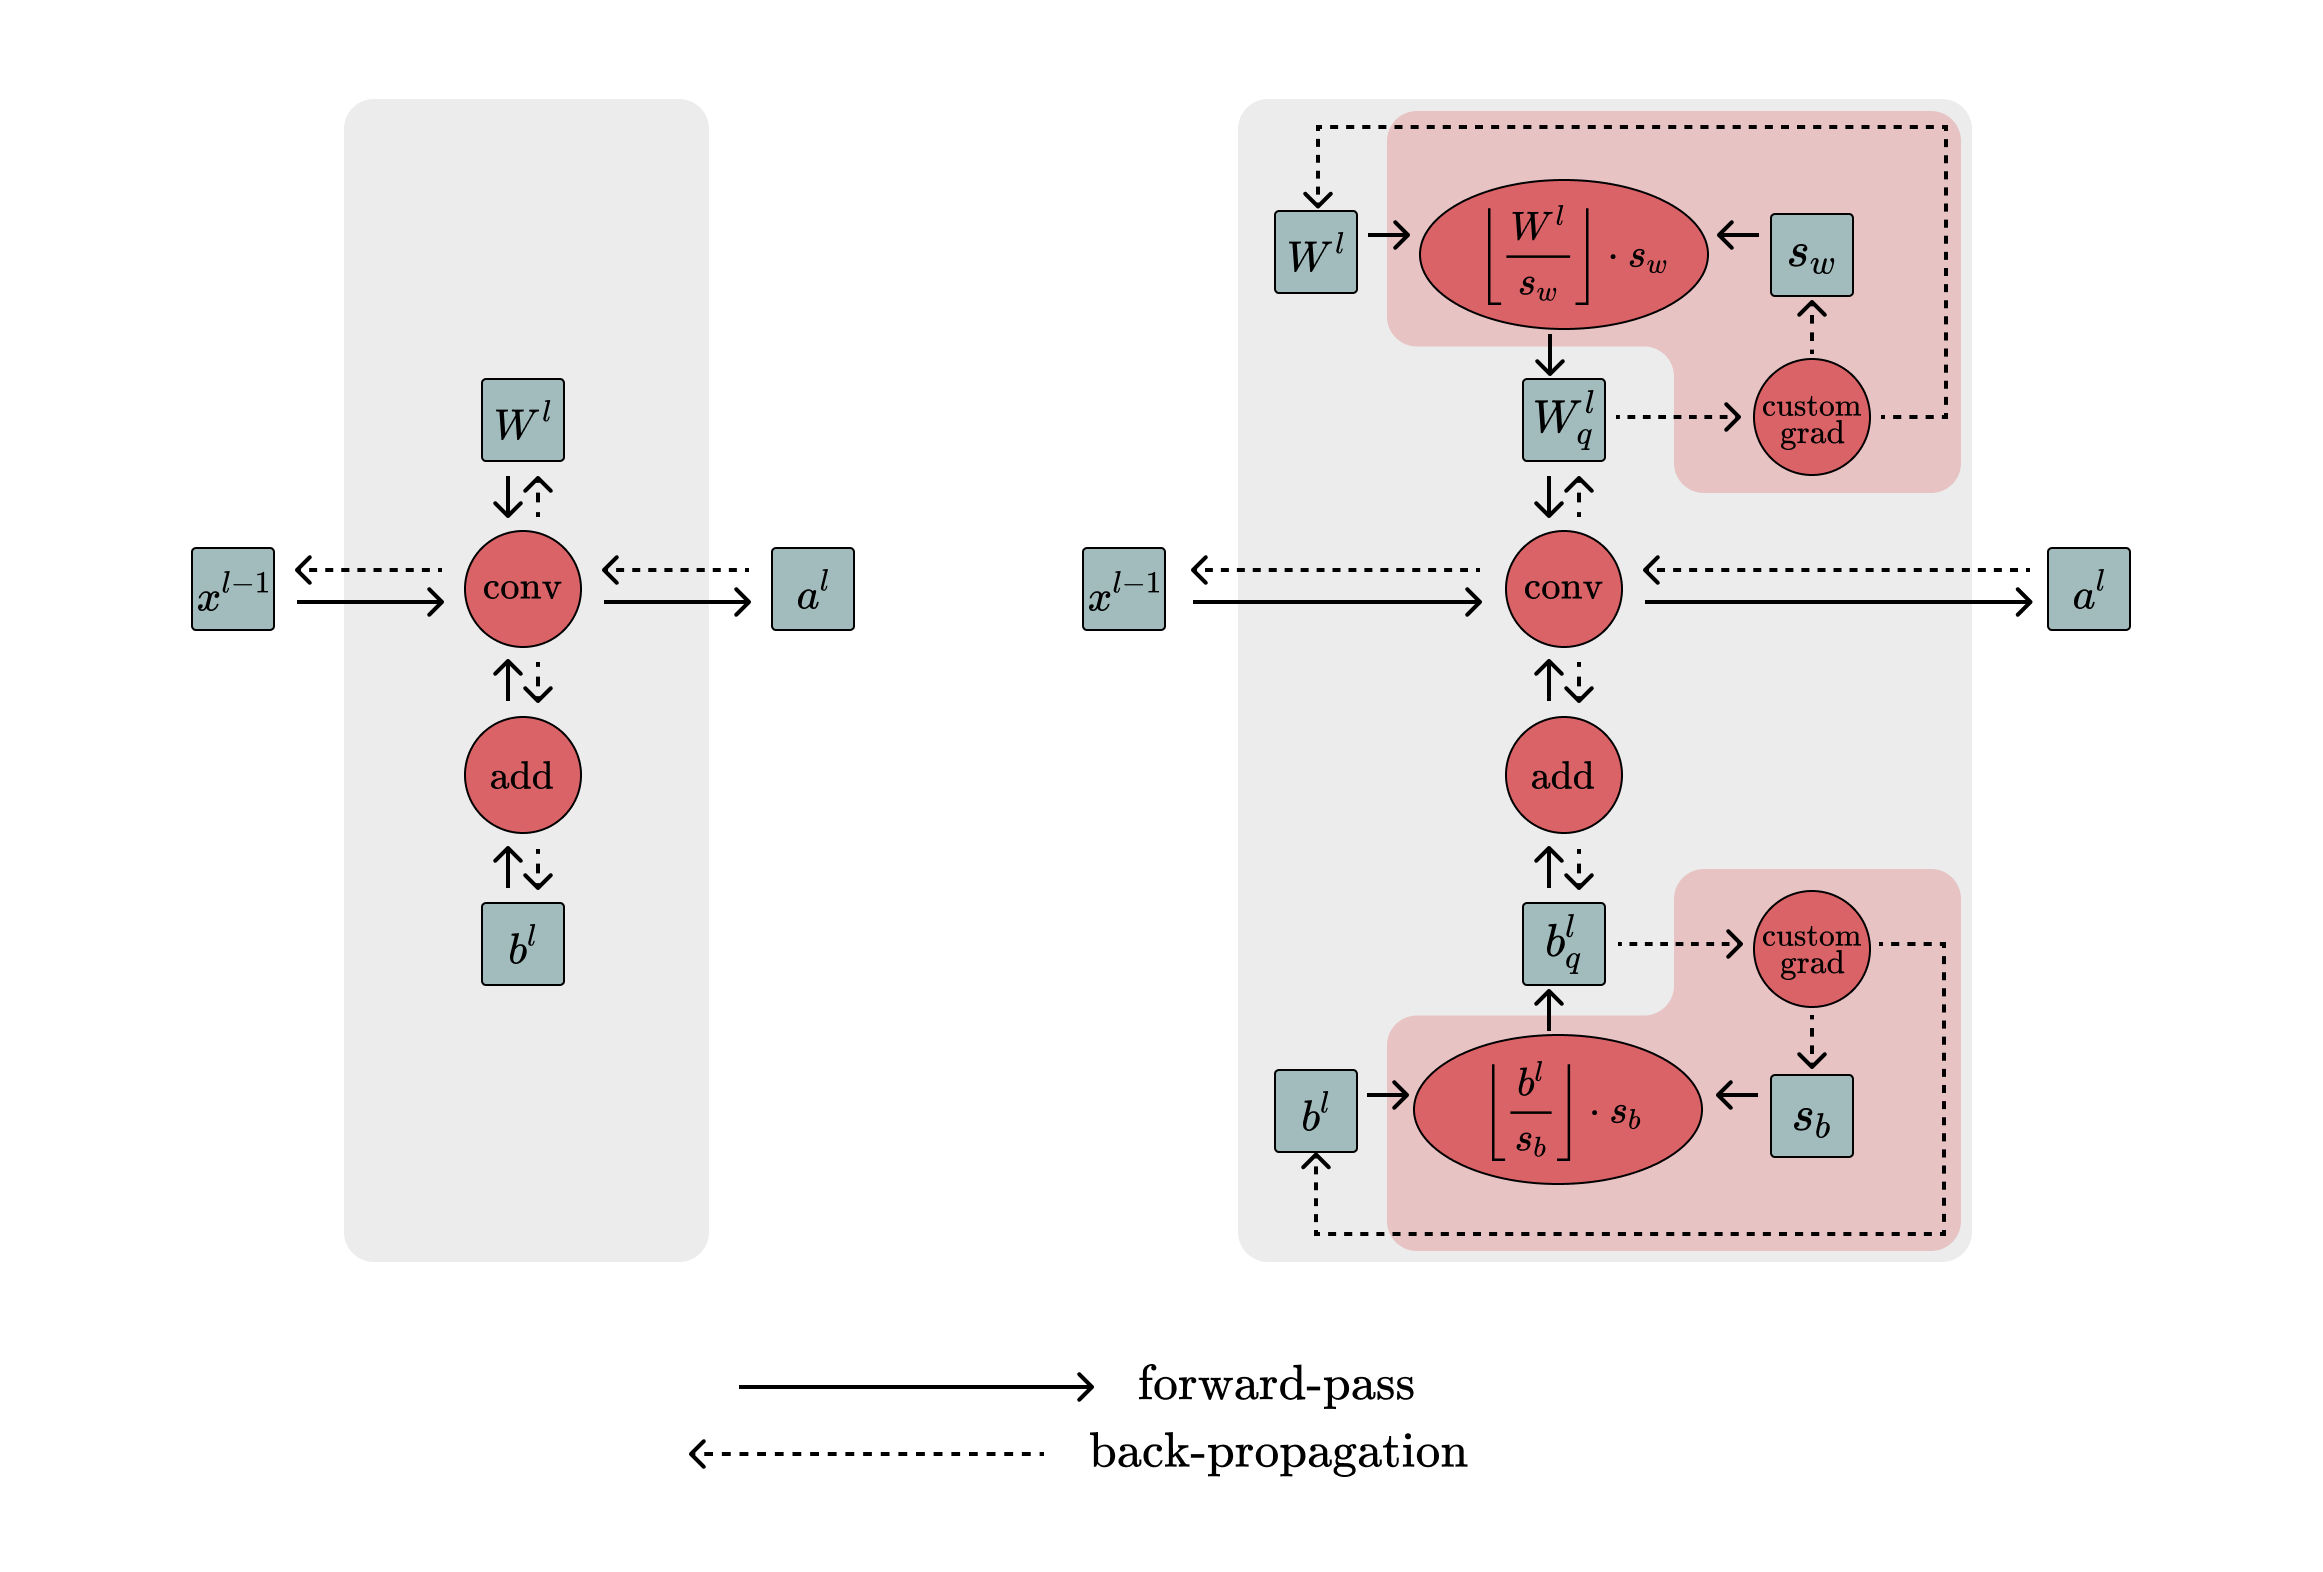
\includegraphics[width=14cm]{nested_quantization_layer.png}
  \caption{A standard convolutional layer (left) and its integration with the nested quantization layer (right) for both weights and bias.
  Quantization logic is applied to weights and biases during the forward pass, with trainable scaling factors 
  updated using custom gradients in the backward pass.}
  \label{fig:dense_layer}
\end{figure}


In this section, we introduce custom layers built upon Tensorflow's \texttt{tf.keras.Layer} class, 
which serves as the base for all Keras layers. Each custom layer also leverages Tensorflow's 
\texttt{tf.custom\_gradient} decorator to define its own gradient computation.
For clarity, the upcoming subsections start by showing how to define the corresponding standard, 
non-quantized layer using \texttt{tf.keras.Layer} and \texttt{tf.customg\_gradient},
then move on to the specific quantized implementations.

Yang You, Igor Gitman, and Boris Ginsburg - Large batch training of convolutional networks
This might have info on the ratio thingie

\section{Custom Loss Functions}
\label{sec:customloss}

\subsection{Penalty for Inverse Scale Factor Magnitude} 
\label{subsec:scaleinverse}

\subsection{Constraint on Bin Count for Quantization}
\label{subsec:maxbin}

\subsection{Deviation between Quantized and Original Values}
\label{subsec:difference}